
\begin{savequote}
The meeting of two personalities is like the contact of two chemical substances: if there is any reaction, both are transformed.
\qauthor{Carl Jung}
\end{savequote}

\chapter[Interpersonal Coordination in NVC]{Interpersonal Coordination in NVC}
\label{ChapterBackchannel}
\label{SectionBackchannelIntro}

\thesiscomment{MAIN POINT OF CHAPTER: Facial behaviour mirroring is observed and quantitatively measured, which provides a basis for automatic \ac{NVC} recognition using backchannel signals.}

\thesiscomment{WHAT we do}

\thesiscomment{HOW we do it}

\thesiscomment{RESULTS, IMPACT and NOVELTY}

The previous chapter considered automatic \ac{NVC} recognition based on visual information of the sender or ``encoder'' of an \ac{NVC} signal (encoder in this case does not refer to the annotators or automatic encoding but rather to the observed subject exhibiting a behaviour \cite{Lanzetta1970}). This chapter considers the behavioural associations between an \ac{NVC} encoder and the \ac{NVC} perceiver, and describes a study of recognising \ac{NVC} signals based on the behaviour of the \ac{NVC} perceiver. In natural two person conversations, the behaviour of one participant influences the other participant. 
%This effect has been previously studied for both verbal and non-verbal communication. 
Usually, people take turns to speak in a conversation. In a dyadic (two person) conversation, the information flow is bi-directional. In a particular speech turn, the speaker's communication is referred to as the ``forward'' channel. The person listening to the speaker also responds to the speaker, primarily using non-verbal communication, and this communication is known as the ``backchannel''. Backchannel communication allows a listener to influence a conversation without verbally interrupting or taking a conversation turn. The forward and backchannel communications occur simultaneously and can vary in style across cultures. For this reason, both subjects in a dyadic conversation can be thought of as both an encoder and perceiver of \ac{NVC} simultaneously and this is bi-directional flow of information exploited in this chapter.

In natural conversations, participants often mimic or mirror behaviours being expressed by the other person. Mimicry or ``behaviour matching'' occurs when two or more people show similar body configurations \cite{Bernieri1991}. For example, if one person touches their face during a conversation, the other person is more likely to do so. 
%This coupling of behaviour is distinct from backchannel communication, because if often occurs without 
Another class of behaviours is performed in a common rhythm, with the starting and ending of movement being simultaneous. This is known as ``synchrony'', which comprises of corresponding rhythms, simultaneous movement and the smooth meshing of interaction \cite{Bernieri1991}. Together, synchrony and behaviour matching are considered as ``interpersonal coordination''. The phenomena of behaviour mirroring and synchrony are not disjunct and can occur at the same time \cite{Delaherche2012}. These effects raises the possibility that a perceiver's behaviour in response to an \ac{NVC} signal may be useful in \ac{NVC} recognition. Based on this idea, backchannel information for automatic \ac{NVC} recognition is studied and evaluated. 

The main contributions of this chapter are:

\begin{itemize}
 \item A method for automatic identification of certain types of interpersonal coordination in the deformation of the face during casual conversation. This method is applied to recorded videos and the results are analysed.
 \item A study of \featureGeneration methods for \ac{NVC} classification that identifies \ac{NVC} signals observed in the forward channel, based solely on backchannel feature data.
\end{itemize}

The next section outlines previous studies that are related to this work. Section \ref{SectionMirrorBehaviour} investigates the inter-person coupling of face deformations in conversation. A automatic system to classify \ac{NVC} based on backchannel cues is described in Section \ref{SectionClassificationBackchannel}.

\section{Related Research}
\label{BackgroundNvcIsCoupled}

Backchannel is a form of human communication which has been relatively little studied. The first mention of it is probably by Yngve \cite{Yngve1970} where he observed that the backchannel allows a listener to express non-verbal or brief verbal speech to influence a conversation, without taking a conversational turn. Even prior to this, gaze was thought to be used in conversation regulation by Kendon \cite{Kendon1967}. Backchannel signals provide a way for a listener to signal agreement or disagreement, as noted by Bousmalis \etal \cite{Bousmalis2009}. Backchannels differ across cultures, with some cultures having a higher frequency of backchannel signals \cite{White1989}.

Human behaviour may also be coupled during conversations, besides consciously performed communication acts. Various studies have tried to quantify this behaviour (see Reidsma \etal \cite{Reidsma2010} and Delaherche \cite{Delaherche2012} for a review). Chartrand and Bargh \cite{Chartrand1999} found that people in conversation tend to adopt the same posture, mannerisms and expression. Similar observations have been found for limb movement, and many aspects of speech, but these effects are dependent on social context \cite{Frith2009}. 
%Patterns in human communication have been studied using automatic means, although this work is at an early stage. 
Several studies have used automatic recognition of synchrony (see \cite{Delaherche2012, Sun2012} for reviews). There is a many different feature extraction techniques and measures of synchrony. Richardson \etal \cite{Richardson2007} studied gaze and noted that when two subjects are observing the same scene, their gaze motion is coupled. They found that behaviour was most strongly coupled between synchronised inter-person movements, but also found evidence of gaze coupling occurring after a delay of up to about 3 seconds. The social situation has an impact on the types of mimicry that occur \cite{Bourgeois2008}. Coupled human behaviour may be useful for automatic recognition. Until recently, there have been no approaches that use backchannel communication. Morency \cite{Morency2011} studied automatic recognition based on backchannel signals and attempted to predict listener responses to a speaker. Okwechime \etal \cite{Okwechime2011} used a-priori data mining to find behaviour patterns in conversation and considered both audio and visual modalities. This study was performed in controlled social situations to elicit interested or disinterested behaviours by the listeners and social context based behaviour differences were identified. %The following section uses geometric features introduced, in the previous chapter, for automatic analysis of coupling of human expression.
Ramseyer and Tschacher \cite{Ramseyer2008} used correlations in difference images to find cross-correlated patterns with a time offset of $\pm$5 sec. They used time shuffled windows to produce non-coordinated behaviour data to determine the extent of cross correlation cause by the null hypothesis. No existing studies consider automatic detection of interpersonal coordination in facial behaviour, although Sun \etal are working towards this goal \cite{Sun2012}.

The MAHNOB HMI iBUG Mimicry dataset (shortened to MHi-Mimicry-db) \cite{Sun2011} contains recordings of dyadic conversations in role play and discussion situations for the purposes of analysing mimicry behaviour. This dataset is significantly larger and more complex than the TwoTalk corpus, containing about 12 hours of records of 40 subjects using 15 video cameras and 3 audio channels. The corpus was manually annotated to produce labels to investigate how mimicry is expressed, if it is intentional or unintentional and the social signal being expressed. Intentional signals were also labelled in terms of the goal of the mimicry. The camera synchronised error was ``well below'' 20 $\mu$sec. The two social situations contained in the MHi-Mimicry-db were a political discussion with a confederate and a role play concerning renting a room to a potential lodger. These scenarios were selected to test specific existing hypothesises of human behaviour. Both were dyadic conversations were conducted in a laboratory. The MAHNOB Mimicry dataset was not available at the time this part of the study was conducted. The following section focuses on interpersonal coordination that may be automatically identified without the use of annotation.

\section{Coupling in Interpersonal Coordination during Informal Conversation}
\label{SectionMirrorBehaviour}

This section describes an automatic method to analyse coupling in facial behaviour. Because this correlation based method is sensitive to both rhythmic and non-rhythmic behaviours, certain types of both mimicry and synchrony behaviours will be detected. Correlation being used as a measure of mimicry can be understood in terms of it's mirroring property. Two people tend to reflect or mirror each others body positions and behaviours. By analogy, correlation is a way of measuring the  extent of ``mirroring'' between two variables. This makes the Peason's correlation suitable for finding some types of coupled behaviours. A more detailed justification of using Pearon's correlation is provided in Appendix \ref{ChapterMimicryColleration}.

Correlation of simultaneous frame features is not sensitive to types of mimicry in which the response behaviour is delayed for a longer time than the duration of the trigger behaviour. The class of behaviours that can be detected by the approach described here will be referred to as ``coupling''. Automatic methods can provide a more comprehensive analysis than can be achieved by manual methods because automatic approaches can scale to large quantities of video data.
% than can be collected by human based encoding (using gesture events, \ac{FACS} or similar). 
%This may be an important as a tool in further research to understand human behaviour. 
The next section describes the method, based on tracking, feature extraction and Pearson correlation. Section \ref{SectionCouplingResults} shows the results and discusses their significance.

\subsection{Methodology}

Using the four dyadic conversations recorded as part of the corpus (see Section \ref{SectionDescriptionOfTwoTalkCorpus}), behaviour patterns that are common to both participants can be identified. The cameras used to record the corpus are genlocked to ensure synchronisation of video frames. Genlock is a common technique to synchronise cameras using a generator signal. The genlock signal was provided by a Tektronix TG700 Multi-Format Video Generator. The cameras were all of the same type; this greatly simplifies achieving accurate synchronisation. Based on informal tests performed by the broadcast engineer responsible for maintaining the system, the camera jitter measured to be was less than one microsecond (the level of jitter in the camera synchronisation was smaller than measurable using the available equipment). The features introduced in the previous chapter are used, \textit{geometric-a}, which are based on distances of pairs of feature trackers (Section \ref{SectionGenerateAlgorithmic}). These features are applied to the face and non-facial behaviour is not considered. %Previous research has found that there are non-facial behaviours that are coupled but this thesis is limited to considering facial behaviour. 
Clearly, some areas of the face will not be coupled e.g. when one person speaks, it is usual for the other person to listen and not to move their mouth in the same way. To identify coupled behaviour, the variation of each feature for both speakers in a conversation are compared using Pearson's correlation $\correlFunc$ (see Equation \ref{EqnPearsonsCorrelation}). If features are highly correlated, this indicates that they are closely coupled. A low correlation indicates the features vary independently. As the correlation is performed on simultaneous frames, it will only capture mimicry between individuals if the offset between the occurrences is less than its duration. While this approach is insensitive to more delayed mimicry, it should identify shorter term mirroring of behaviour (see Appendix \ref{ChapterMimicryColleration}). The correlation score corresponds to the strength of coupling of the behaviour. The original video records are used because it increases the quantity of data available for analysis. The feature vectors $\frameFeatureMatrix$ of two participants $A$ and $B$ are compared $A, B \in \{1008, 1011, 2008, 2011, 3008, 3011, 6008, 6011\}$. For feature component $i \in \{0...\numFeatures\}$, the correlation $\dyadicCorrelation$ is ($\frameFeatureMatrix^A_i \in \mathbb{R}^{\numSeqFrames}$, $\numSeqFrames = 12 \times 60 \times 25 frames$, $\dyadicCorrelation^{A,B}_i \in \mathbb{R}$):

\begin{gather}
\dyadicCorrelation^{A,B}_i = \correlFunc(\frameFeatureMatrix^A_i, \frameFeatureMatrix^B_i)
\end{gather}

If a behaviour is performed as a reaction, there may be a time delay between the behaviours. Each frame of one participant is compared to a simultaneous frame of the other participant taken using a second camera. This makes this approach sensitive to synchronised behaviours but insensitive to mirroring behaviours that have a temporal offset and short duration. For example, if one person adopts an expression for several seconds and the second person quickly adopts the same expression, this will be found using the correlation of features. The correlation coefficient is limited to measuring linear relationships. It is quite possible that reliable, non-linear patterns of human behaviour may exist. Another limitation of this approach is that this considers only variations in shape but it is possible that patterns in human behaviour may be found if speed or acceleration of the face is also considered.

For this test, corresponding features are compared (e.g. position of left eye in both participants) rather than different areas on the face (e.g. left eye for one subject and mouth opening for the second subject). This constraint makes the system focus primarily on mirroring behaviour. Because the strongly coupled areas of the face are most interesting, the highest scoring feature $i^{A,B}_{max}$, with correlation $\dyadicCorrelation^{A,B}_{max}$, is found:

\begin{gather}
i^{A,B}_{max} = \argmax_{i}{\dyadicCorrelation^{A,B}_i}
\end{gather}

This feature corresponds to a specific area on the face in which the behaviour is coupled. However, there is a possibility that features vary and may coincidentally vary together. It can be difficult to distinguish weak causal relationships with coincidental inter-relationships. To examine this possibility, the correlations of features $\dyadicCorrelation_{max}$ for individuals that were not in the same conversation was also computed. Apparent correlations between unrelated conversations can be regarded as coincidental.
%, except if there is a inter-conversation pattern. An example of patterns that occur across conversation might be if head position varies in time due to tiredness. However, it is thought that this effects will not be significant compared to intentional gestures.

%The next section presents the results of this approach and discusses their significance.

This method is similar to Ramseyer and Tschacher \cite{Ramseyer2008} but contains some important differences:
\begin{itemize}
 \item This study uses face shape based on tracking rather than difference images of whole people. This makes our approach more effective in localising coupling behaviour to a specific area of the face. However, no other areas of the body are considered in this study.
 \item This study uses recordings of a different person to test the null hypothesis correlations, rather than a shuffled window approach. However, this should not give rise to a significant difference in measured performance.
 \item Ramseyer and Tschacher considered time offset signals, which enabled them to see which person is leading and which person is following in behaviour. This is not attempted in this study.
\end{itemize}

The current section only aims to show that interpersonal coordination exists for some areas of the face in dyadic informal conversation. Therefore, this study consider pairs of participant independently but without attempting to find consistent behaviour patterns that occur in all dyads. This approach of considering dyads independent and without finding corresponding behaviours across dyads was also used by Ramseyer and Tschacher \cite{Ramseyer2008}. 
%Okwechime \etal used only a single triadic discussion for finding behaviour patterns \cite{Okwechime2011}. 
Although attempting to find consistent behaviours from multiple dyads would be an interesting study, it is beyond the scope of this thesis. 

\subsection{Results and Discussion}
\label{SectionCouplingResults}

\thesisstatement{A method for automatic identification of coupled movements and deformations of the face during casual conversation. The couple areas for the TwoTalk corpus are shown.}

\begin{table}[tb]
\centering
\caption{Maximum correlation $\dyadicCorrelation_{max}$ of corresponding facial shape features for different pairs of participants. Pairs that were participating in the same conversation are highlighted.}
\begin{tabular}{ | c | c | c | c | c | c | c | c | c |}
\hline
& 1008 & 1011 & 2008 & 2011 & 3008 & 3011 & 6008 & 6011 \\
\hline
1008 & \cellcolor{orange} 1.00 & \cellcolor{orange} 0.25 & 0.12 & 0.11 & 0.15 & 0.13 & 0.08 & 0.10\\
1011 & \cellcolor{orange} & \cellcolor{orange} 1.00& 0.19& 0.13& 0.18& 0.10& 0.15& 0.21\\
2008 & & & \cellcolor{orange} 1.00& \cellcolor{orange} 0.38& 0.11& 0.16& 0.12& 0.14\\
2011 & & & \cellcolor{orange} & \cellcolor{orange} 1.00 & 0.14& 0.18& 0.13& 0.12\\
3008 & & & & & \cellcolor{orange} 1.00 & \cellcolor{orange} 0.34& 0.09&0.20\\
3011 & & & & & \cellcolor{orange} & \cellcolor{orange} 1.00& 0.09& 0.09\\
6008 & & & & & & & \cellcolor{orange} 1.00& \cellcolor{orange} 0.38\\
6011 & & & & & & & \cellcolor{orange} & \cellcolor{orange} 1.00\\
\hline
\end{tabular}
\label{TableBackchannelShapePairs}
\end{table}

The maximum correlation $\dyadicCorrelation_{max}$ of different pairings of subjects is shown in Table \ref{TableBackchannelShapePairs}. The conversation pairs are shown in Table \ref{ParticipantDemographics}. There is a weak but significant correlation (between 0.25 and 0.38) for pairs involved in the same conversation. This confirms our expectation that there are interpersonal coordinated behaviours for corresponding areas of the face. Comparing this to conversation pairings in which the correlation would be coincidental, the correlation is found to be consistently lower than 0.25. This implies that the coupling of facial behaviour in conversation is above the level of correlation due to coincidental matches. Not all highlighted conversation pairs have the same level of correlation. This may be due to different relationships and communication styles between conversation participants. There may be person specific differences in their tendency to couple behaviour, as found by Chartrand and Bargh \cite{Chartrand1999}.

\begin{figure}[tb]
\centering
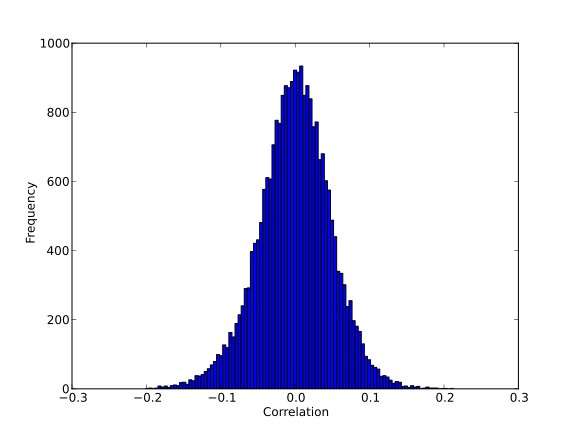
\includegraphics[width = 0.8 \columnwidth]{backchannel/correlationHist.pdf}

\caption[Histogram of correlation for corresponding algorithmic geometric features that originate from \textit{different} conversations.]{Histogram of correlation for corresponding algorithmic geometric features that originate from \textit{different} conversations. The standard deviation is 0.048 and the variance is 0.002.}
\label{FigureCorrelationHist}
\end{figure}

The statistical significance of the best correlated features can be confirmed by characterising the distribution of correlation performance scores for the null hypothesis and use it to calculate the p-value for the hypothesis of interest. The possibility of a null hypothesis can be discounted if this p-value is lower than the desired significance level $\alpha$ and can then be considered as statistically significant (see Hayes \cite{Hayes2005}). Because multiple hypothesises are tested, $\alpha$ is adjusted using the Bonferroni correction to account for the greater chance of finding coincidental patterns. Any correlations between feature pairs that originate from separate conversations are due to chance. The distribution of correlation scores for null hypothesis pairings is shown in Figure \ref{FigureCorrelationHist}. The standard deviation of correlation scores from null hypothesis pairings is $\sigma=0.048$ and the variance is $\sigma^2=0.002$. The chance correlation distribution is zero centred $\bar{\correlFunc}=0$. The p-value of a correlation score $\correlFunc$ is calculated by a z-test. A z-test is used because the standard deviation of all possible null hypothesis is known. For a single observation compared to a zero centred population $\bar{\correlFunc}=0$, the z-test score is defined as:

\begin{gather}
z = \frac{\correlFunc}{\sigma}
\end{gather}

For the highest correlation by chance, $\correlFunc=0.21$, the corresponding z-score is $z=-0.21/0.048=−4.4$ and p-value is $2\times\mathcal{N}(−4.4)=1.2\times10^{-5}$ where $\mathcal{N}$ is the cumulative normal distribution. The double tailed score is used because the modulus of the correlation is used to determine the largest magnitude correlation. The standard significance level $\alpha$ is usually chosen to be either $0.01$ or $0.05$. The more stringent level $\alpha=0.01$ is used in this chapter. Each of the correlation scores use the maximum value, based on 1035 comparisons (see Section \ref{SectionGenerateAlgorithmic}). The Bonferroni corrected $\alpha$ is calculated as $\alpha_{adjusted} = \frac{0.01}{1035}=9.7\times10^{-6}$. The p-value of $1.2\times10^{-5}$, observed in the validation experiments, is within this threshold and cannot be considered as a statistically significant finding, as should be expected. 

For pairings in which are engaged in the same conversation, patterns that are clearly statistically significant are expected. The correlation scores for these conversations vary from $\correlFunc=0.25$ to $\correlFunc=0.38$. This corresponds to p-values between $2\times\mathcal{N}(-0.25/0.048)=1.9\times10^{-7}$ and $2\times\mathcal{N}(-0.38/0.048)=2.4\times10^{-15}$, respectively. These are well below the Bonferroni corrected significance level of $9.7\times10^{-6}$. The null hypothesis may therefore be rejected for these tests and they are therefore statistically significant.

\begin{figure}[tb]
\centering
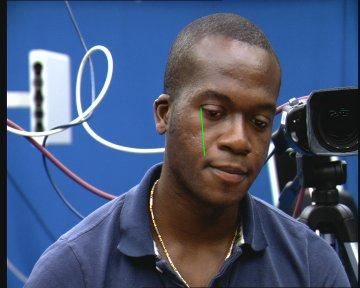
\includegraphics[width = 0.49 \columnwidth]{backchannel/1008.pdf}
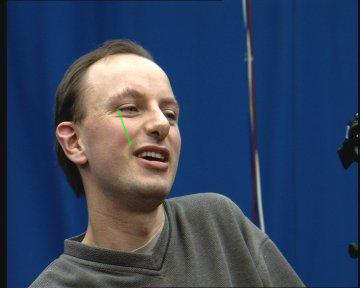
\includegraphics[width = 0.49 \columnwidth]{backchannel/1011.pdf}

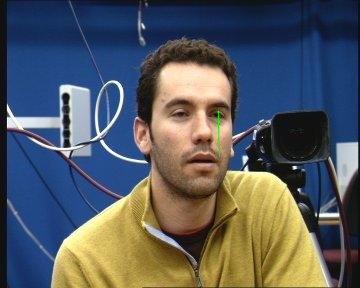
\includegraphics[width = 0.49 \columnwidth]{backchannel/3008.pdf}
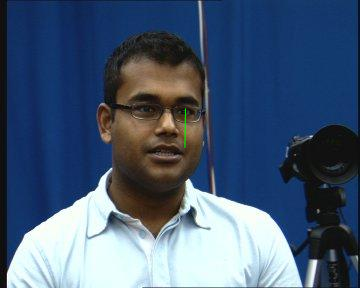
\includegraphics[width = 0.49 \columnwidth]{backchannel/3011.pdf}
\caption[Corresponding facial distances found to be most coupled in natural conversation for two of the conversations, marked in green.]{Corresponding facial distances found to be most coupled in natural conversation for two of the conversations, marked in green. The top row is conversation 1008-1011. The bottom row is conversation 3008-3011.}
\label{BackChannelCoupledPose}
\end{figure}

\begin{figure}[tb]
\centering
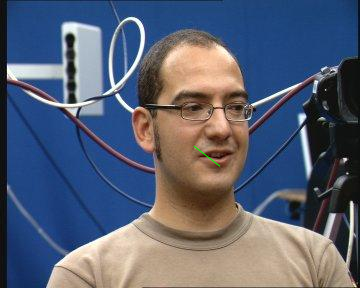
\includegraphics[width = 0.49 \columnwidth]{backchannel/2008.pdf}
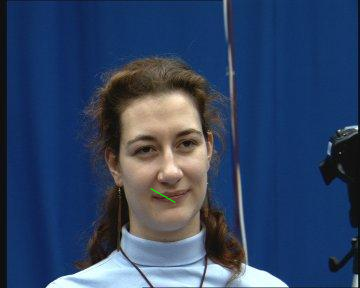
\includegraphics[width = 0.49 \columnwidth]{backchannel/2011.pdf}

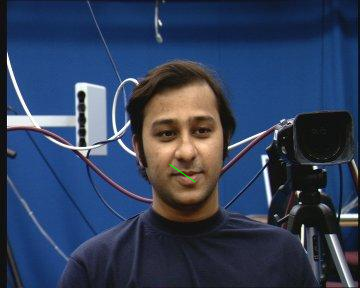
\includegraphics[width = 0.49 \columnwidth]{backchannel/6008.pdf}
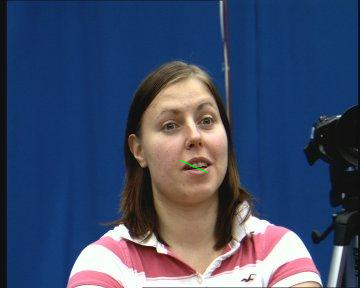
\includegraphics[width = 0.49 \columnwidth]{backchannel/6011.pdf}
\caption[Corresponding facial distances found to be most coupled in natural conversation for two of the conversations, marked in green.]{Corresponding facial distances found to be most coupled in natural conversation for two of the conversations, marked in green. The top row is conversation 2008-2011. The bottom row is conversation 6008-6011.}
\label{BackChannelCoupledMouth}
\end{figure}

The two areas of the face found to be coupled in natural conversation are shown in Figures \ref{BackChannelCoupledPose} and \ref{BackChannelCoupledMouth}. The areas shown in Figure \ref{BackChannelCoupledPose} seem to involve vertical distances which are generally rigid and likely encode head pitch. In contrast, the second group's relevant areas, shown in Figure \ref{BackChannelCoupledMouth}, are more related to the mouth and perhaps relate to mutual smiling or some other mouth related expression.
%1011,1008,0.248663511096,886,886 10045-488 P
%2011,2008,0.384282031869,903,903 10119-488 M
%3011,3008,0.343704739655,230,230 6249-1924 P
%6011,6008,0.375698211625,661,661 6718-488 M
The next section attempts to find patterns in facial behaviour that are not necessarily related to corresponding areas of the face.

\subsection{Coupling of Shape for Non-corresponding Facial Features}

\begin{table}[tb]
\centering
\caption[Maximum correlation $\dyadicCorrelation_{max}$ of \textbf{facial shape features} for different pairs of participants (including corresponding and non-corresponding features).]{Maximum correlation $\dyadicCorrelation_{max}$ of \textbf{facial shape features} for different pairs of participants (including corresponding and non-corresponding features). Pairs that were participating in the same conversation are highlighted.}
\begin{tabular}{ | c | c | c | c | c | c | c | c | c |}
\hline
& 1008 & 1011 & 2008 & 2011 & 3008 & 3011 & 6008 & 6011 \\
\hline
1008 & \cellcolor{orange} 1.00 & \cellcolor{orange} 0.30 & 0.18 & 0.15 & 0.23 & 0.22 & 0.15 & 0.18\\
1011 & \cellcolor{orange} & \cellcolor{orange} 1.00& 0.25& 0.22& 0.29& 0.23& 0.21& 0.23\\
2008 & & & \cellcolor{orange} 1.00& \cellcolor{orange} 0.43& 0.17& 0.23& 0.17& 0.18\\
2011 & & & \cellcolor{orange} & \cellcolor{orange} 1.00 & 0.22& 0.19&0.18 &0.19 \\
3008 & & & & & \cellcolor{orange} 1.00 & \cellcolor{orange} 0.49& 0.18& 0.29\\
3011 & & & & & \cellcolor{orange} & \cellcolor{orange} 1.00& 0.21& 0.16\\
6008 & & & & & & & \cellcolor{orange} 1.00& \cellcolor{orange} 0.42\\
6011 & & & & & & & \cellcolor{orange} & \cellcolor{orange} 1.00\\
\hline
\end{tabular}
\label{TableBackchannelShape}
\end{table}

The previous section considered the interpersonal coordination of facial behaviour for corresponding areas of the face. However, facial behaviour coupling between people may be expressed in different facial areas. This falls within the definition of synchrony, for which ``the important element is the timing, rather than the nature of the behaviours'' \cite{Delaherche2012}. Synchrony can involve coordinated times of different forms of behaviour, e.g. beginning to speak when another person stops speaking. This phenomena has been explored to some extent by Ramseyer and Tschacher \cite{Ramseyer2008}, who did not use corresponding parts of the body but instead searched entire images for any movement synchrony. To find correlations for this broader problem, the feature component $i$ for subject $A$ is compared to feature component $j$ for subject $B$. Because each feature component corresponds to a different area of the face, this searches for relationships in shape between non-corresponding facial areas. The correlation between facial components $i$ and $j$ ($i \in \{0...\numFeatures\}$ and $j \in \{0...\numFeatures\}$) defined as $\dyadicCorrelation^{A,B}_{i,j} \in \mathbb{R}$ for subject $A$ and $B$:

\begin{gather}
\dyadicCorrelation^{A,B}_{i,j} = \correlFunc(\frameFeatureMatrix^A_i, \frameFeatureMatrix^B_j) \\
(i_{max}, j_{max}) = \argmax_{i,j}{\dyadicCorrelation^{A,B}_{i,j}}
\end{gather}

Again, the components $i_{max}, j_{max}$ with the highest correlation $\dyadicCorrelation^{A,B}_{i,j}$ are determined. The result of this process is shown in Table \ref{TableBackchannelShape}. The correlation for pairs in the same conversation is consistently above the correlation of coincidence matches. The standard deviation of correlation scores from null hypothesis pairings is $0.047$ and the variance is $\sigma^2=0.002$, which is similar to the case of chance correlations if only corresponding features are considered (see Figure \ref{FigureCorrelationHist}). More comparisons are performed to obtain the maximum correlation for each pair of subjects. This results in a more stringent Bonferroni adjusted $\alpha$, which is calculated as $\alpha_{adjusted} = \frac{0.01}{T_{1035-1}}=1.87\times10^{-8}$ where $T_i$ is the $i$th triangular number. For pairs of subjects in engaged in conversation, the maximum correlation for each pair is 0.30, 0.43, 0.49 and 0.42. Based on the z-test, these correlations have a p-value of $1.7\times10^{-10}$, $5.75\times10^{-20}$, $1.90\times10^{-25}$ and $4.03\times10^{-19}$ respectively. The first is relatively near the significance boundary, while the latter three results are clearly statistically significant. There may be because the broader range of facial areas considered includes a wider range of human expression, so instead of just co-occurrence behaviours, other strongly coupled communication relationships can be detected. Because a greater number of feature components are compared, there is an increased possibility for coincidental matches. This is evident in the table because the off axis pairings show an increase in correlation compared to Table \ref{TableBackchannelShapePairs}. These results indicate that some facial behaviour is coupled and this coupling is stronger if non-corresponding facial areas are also considered. Although the correlation scores are above chance occurrence, they are not perfectly consistent patterns of human behaviour. This does not make this patterns uninteresting or insignificant because most inter-personal behaviours are only general patterns; identification of deterministic patterns in human behaviour are not the norm.

%So far in this chapter, coupling of face deformation has been investigated. The next section considers behaviour coupling based on variation of face shape in a sliding window.

\subsection{Coupling of Facial Shape Activity for Non-corresponding Facial Features}

\begin{table}[tb]
\centering
\caption[Maximum correlation $\dyadicCorrelation_{max}$ of sliding window \textbf{variance of facial shape}, for various pairs of participants (including corresponding and non-corresponding features).]{Maximum correlation $\dyadicCorrelation_{max}$ of sliding window \textbf{variance of facial shape}, for various pairs of participants (including corresponding and non-corresponding features). Pairs that were participating in the same conversation are highlighted.}
\begin{tabular}{ | c | c | c | c | c | c | c | c | c |}
\hline
& 1008 & 1011 & 2008 & 2011 & 3008 & 3011 & 6008 & 6011 \\
\hline
1008 & \cellcolor{orange} 1.00& \cellcolor{orange} 0.32& 0.13& 0.13& 0.29& 0.38& 0.16& 0.27\\
1011 & \cellcolor{orange} & \cellcolor{orange}1.00& 0.33& 0.21& 0.19& 0.16& 0.21& 0.18\\
2008 & & & \cellcolor{orange} 1.00& \cellcolor{orange}0.34& 0.11& 0.23&0.16 &0.21 \\
2011 & & & \cellcolor{orange} & \cellcolor{orange}1.00 & 0.12& 0.14& 0.26& 0.29\\
3008 & & & & & \cellcolor{orange}1.00& \cellcolor{orange}0.41& 0.47& 0.14\\
3011 & & & & & \cellcolor{orange} & \cellcolor{orange}1.00& 0.27& 0.25\\
6008 & & & & & & & \cellcolor{orange}1.00&\cellcolor{orange} 0.15\\
6011 & & & & & & & \cellcolor{orange} & \cellcolor{orange}1.00\\
\hline
\end{tabular}
\label{TableBackchannelVar}
\end{table}

The previous sections have examined coupling of face shape in natural, dyadic conversation. However, it may be that facial motion contains reliable patterns of human behaviour. For instance, head pitch activity might encode nodding in agreement and this may be related to mouth activity caused by talking. The variance of each feature component in a sliding window was calculated. The window was selected to be 1 second in duration (25 frames), because this is sensitive to \ac{NVC} signals of a relatively short duration. However, different \ac{NVC} signals may occur on other time scales which would not be detected. At sliding window position $\timeOffset$, the variance $\slidingWindowVar$ of a feature component in a sliding window of 25 frames duration is:

\begin{gather}
\label{EqnVarianceSlidingWindow}
\slidingWindowVar^A_{\timeOffset,i} = \frac{1}{25} \displaystyle\sum\limits^{12}_{a=-12} {\frameFeatureMatrix^A_{\timeOffset+a,i}}^2 - \left( \frac{1}{25}\displaystyle\sum\limits^{12}_{a=-12} {\frameFeatureMatrix^A_{\timeOffset+a,i}} \right)^2\\
\dyadicCorrelation^{A,B}_{i,j} = \correlFunc(\slidingWindowVar^A_i, \slidingWindowVar^B_j)
\end{gather}

The results of this method are shown in Figure \ref{TableBackchannelVar}. In this case, the correlations caused by coincidence (shown in the off axis pairings) are often higher than the correlations that might be expected to have coupling. The variance of correlations from null hypothesis pairings has a standard deviation of $0.034$. For subject pairs engaged in conversation, the maximum correlations were 0.32, 0.34, 0.41 and 0.15. Based on the z-test, the p-values for these results are $4.88\times10^{-21}$, $1.52\times10^{-23}$, $1.74\times10^{-33}$ and $1.03\times10^{-05}$ respectively. The first three pairings are well below the significance threshold $\alpha_{adjusted} = \frac{0.01}{T_{1035-1}}=1.87\times10^{-8}$ but the final pair is above the threshold and is more likely to be due to a null hypothesis. The highest correlation is for conversation 3008-6008 which has $\dyadicCorrelation=0.47$ and is caused by coincidental variation of the features (p-value $1.84\times10^{-43}$). This coincidental match is strangely below the significance threshold and may be due to the distribution of correlations being non-Gaussian. Since coupling cause by patterns in human behaviour cannot be distinguished from those cause by coincidence, more data is required to obtain results that can be confidently considered as statistically significant. An analysis of facial shape activity based on corresponding features resulted in a similar, non-significant result and has been omitted for brevity. This system was not compared to human performance for identifying interpersonal coordination because the resources required to collect such an annotation data set would be very resource intensive and this is beyond the scope of this thesis.
Facial shape in natural conversations exhibits interpersonal coordination. Given the relationship between people's behaviours, the next section uses backchannel information for automatic \ac{NVC} recognition. However, the following section considers all feature components rather than the components identified in earlier in the chapter. This allows features to be used in the classifier model that do not necessarily have a linear coupling with the forward channel behaviour.

\section{Classification Based on Backchannel Information}
\label{SectionClassificationBackchannel}

The previous chapter has investigated automatic methods to classify \ac{NVC} based on visual facial information. However, the corpus has two subjects interacting. The annotated subject is designated as the ``sender'' and the other conversation participant as the ``receiver''. 
The sender expresses in the forward channel and perceives the backchannel. The receiver expresses in the backchannel and perceives the forward channel. 
The previous section has discussed coupling of facial behaviour in natural conversation. This raises the possibility that a sender's \ac{NVC} signals may be inferred based on the receiver's visual information. Figure \ref{BackChannelFigure} shows the experimental arrangement to detect \ac{NVC} using backchannel signals. The videos of \ac{NVC} receiver participants are tracked and features extracted using \textit{geometric-a} features, as described in Section \ref{SectionGenerateAlgorithmic}. A classifier is trained on the sender \ac{NVC} labels and the receiver facial feature data. Testing is performed on a person independent basis, with only clear \ac{NVC} clips used in the test $\clearClipSet^{clear}_{\nvcCategory}$ (see Section \ref{SectionClearExamples}) based on annotation ratings of the \ac{NVC} sender. %Test features are used to train an \ac{SVM} classifier.

\begin{figure}[tb]
\centering
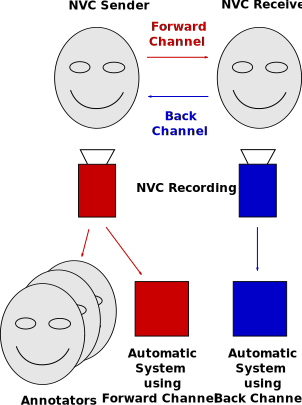
\includegraphics[width = 0.4 \columnwidth]{backchannel/figureforwardbackchannel.pdf}
\caption{Automatic \ac{NVC} classification can operate on either the forward or backchannel information.}
\label{BackChannelFigure}
\end{figure}

The experimental arrangement is almost identical to that presented in the previous chapter. The target classes and annotation data is described in Chapter \ref{ChapterCorpus}. \FeatureGeneration is performed as discussed in Section \ref{SectionFeatureGeneration}. Classification is performed as described in Section \ref{SectionClassificationMethods}. Eight fold cross validation is used on clear examples of \ac{NVC} (Section \ref{SectionClearExamples}) and performance is evaluated using \ac{AUC}, as described in Section \ref{SectionClassificationPerformance}. The only difference is the shape features used for training and testing are taken from the other person in the dyad (i.e. the person conversing with the subject that was shown to the annotators).

\subsection{Results and Discussion}

\thesisstatement{Classification of NVC is possible from backchannel signals but is more difficult than forward channel.}

\thesisstatement{Algorithmic features are good at generalising to the person independent NVC classification and regression (for forward and backchannel signals)}

The performance of automatic classification based on backchannel \ac{NVC} signals is shown in Table \ref{TableBackchannel}. If the performance for forward channel \ac{NVC} classification (Table \ref{TableCompareFeaturesAndClassifiers}) is compared to backchannel performance, it can be seen that the backchannel performance is equal or lower in every case. This is unsurprising, because backchannel information is only a behavioural response to forward channel communication. The results suggest that, for some methods of \featureGenerationComma the classifier is consistently performing at above chance level of 0.5. However, additional tests are required to establish if this result is statistically significant. If the performance for each of the \featureGeneration methods is compared, it can be seen that \textit{geometric-a} features are again the most effective. The majority of other feature sets have performance levels at or near chance level. Person independent testing is more challenging than multi-person testing in all cases. 
%The best performing features are geometric based with \textit{geometric-h} has a larger drop moving from multi-person to person independent. 
These observations have the same general pattern as the forward channel performance results.

\begin{table}[tb] % XIV, XII, XV, XIII
\centering
%\rowcolors[]{1}{white!20}{white!10} 
\caption{\ac{AUC} \ac{ROC} performance using backchannel features (clip level testing, person independent testing, average score of categories and average standard deviation from Tables \ref{BoostClipMultipersonReceiverTable} to \ref{SvmClipPersonindepReceiverTable} are shown).}
\begin{tabular}{ c | c | c | c | c }
\hline
Test & \multicolumn{2}{c|}{Multi-person} & \multicolumn{2}{c}{Person independent} \\
 & SVM & Adaboost & SVM & Adaboost \\
\hline
affine                           & 0.50 $\pm$ 0.04 & 0.53 $\pm$ 0.05 & 0.49 $\pm$ 0.05 & 0.50 $\pm$ 0.04 \\
deform-cubica                    & 0.51 $\pm$ 0.01 & 0.52 $\pm$ 0.05 & 0.50 $\pm$ 0.00 & 0.49 $\pm$ 0.06 \\
deform-fastica                   & 0.51 $\pm$ 0.01 & 0.52 $\pm$ 0.05 & 0.50 $\pm$ 0.00 & 0.49 $\pm$ 0.06 \\
deform-pca                       & 0.54 $\pm$ 0.04 & 0.62 $\pm$ 0.07 & 0.50 $\pm$ 0.00 & 0.52 $\pm$ 0.04 \\
geometric-h                      & 0.65 $\pm$ 0.05 & 0.66 $\pm$ 0.07 & 0.54 $\pm$ 0.04 & 0.59 $\pm$ 0.07 \\
\rowcolor[gray]{.95} geometric-a & 0.67 $\pm$ 0.03 & 0.68 $\pm$ 0.09 & 0.59 $\pm$ 0.08 & 0.59 $\pm$ 0.09 \\
lbp                              & 0.54 $\pm$ 0.05 & 0.58 $\pm$ 0.05 & 0.49 $\pm$ 0.07 & 0.48 $\pm$ 0.10 \\
lm                               & 0.55 $\pm$ 0.03 & 0.56 $\pm$ 0.06 & 0.48 $\pm$ 0.02 & 0.50 $\pm$ 0.05 \\
\hline
\end{tabular}
\label{TableBackchannel}
\end{table}

One difference between backchannel and forward channel is that \ac{SVM} classification has equal to or worse performance when compared to Adaboost. This may be due to over fitting of the SVM, which might be addressed by parameter tuning.

%The next section draws general conclusions based on the chapter's results.

\section{Conclusion}

This chapter has identified coupled behaviour in facial expression and described a study of backchannel features to classify forward channel \ac{NVC}. This was based on previous research that found many human behaviours are inter-personally coordinated in two person conversations. Coupled facial deformations were identified for both corresponding regions of the face, as well as non-corresponding regions. The corresponding areas are situated in the mouth area or were thought to relate to head pitch. Classification was also possible using backchannel features, although the performance is significantly lower if compared to forward channel features. 

This area of research is still at an early stage. There are many potential improvements and extensions to the work presented in this chapter. For instance, coupled behaviours were only examined in conversation pairs, which may lead to personal differences in behavioural patterns. It would be possible to modify the method to look for behavioural patterns that consistently occur across a larger group of conversation participants. Also, only instantaneous face deformations were considered. If an effective way of encoding face deformation or gesture was found, it may be possible to check for responses to stimuli that occur after a time delay, in a similar fashion to Richardson \etal \cite{Richardson2007}. Pearson's correlation coefficient is only sensitive to linear correlations between variables, but it is quite possible that non-linear behavioural patters may exist. Only facial deformation is considered in the features and it would be interesting to expand the behavioural encoding to verbal communication, as well as arm position and body pose. This would enable a much broader range of social phenomena to be studied.

There are also possible extensions to classification based on backchannel features. It should be possible to combine backchannel and forward channel features, either by feature or decision fusion, to improve performance. Also, many of the limitations of the previous chapter apply here: \ac{NVC} is not temporally modelled, and the social context and cultural background of the participants and annotators could be better controlled. To address the cultural differences of the annotators, the next section describes the collection of a \culturallySpecific annotation set for the TwoTalk corpus.

